% ==============================================================================
% chapters/ch06_delivery_wall_resilience.tex
% פרק ו': בחינת עמידות המערכת הבנקאית והיזמית לקראת "קיר המסירות" (2026–2027)
% ==============================================================================

\chapter{בחינת עמידות המערכת הבנקאית והיזמית לקראת \en{"}קיר המסירות\en{"} (\num{2026}--\num{2027})}
\label{ch:delivery_wall_resilience}

פרק זה מציג את הממצאים האנליטיים הראשוניים מהרצת מערך הסימולציות ומבחני הקיצון שפותחו בפרק ה', ומעניק מענה כמותי ישיר לחלקה השני של שאלת המחקר המרכזית: **מהי עמידות המערכת הבנקאית והיזמית בישראל בפני גל חדלות פירעון בעת \en{"}קיר המסירות\en{"} של שנות \num{2026}--\num{2027}?** הממצאים מאמתים את השערות המחקר ($H_1, H_2, H_3$) וחושפים תמונת עמידות דו-קוטבית: בעוד שליבת המערכת הבנקאית המסחרית בישראל מפגינה חוסן יוצא דופן ושומרת על יחס הון \en{CET1} מעל הרף הרגולטורי גם בתרחיש הקיצון החמור ביותר, הרי שבקרב משקי הבית שרכשו במבצעי מימון ובקרב יזמים מדרג \en{Tier-2} ו-\en{Tier-3} הממונפים באשראי חוץ-בנקאי, קיר המסירות צפוי לחולל זעזוע נזילות וגל כשלי סגירה משמעותי.

\section{עמידות משקי הבית: תוצאות סימולציית המונטה-קרלו להלם ההחזר (\en{Payment Shock})}
\label{sec:resilience_households}

איור~\ref{fig:payment_shock_mc} מציג את התפלגות יחס ההחזר להכנסה פנויה (\en{PTI}) של $N = 10,000$ משקי בית בסימולציית המונטה-קרלו (המייצגים את \num{54,200} משקי הבית בפלח ה-\en{SOM} שרכשו דירות במבצעי \num{20/80}, \num{10/90} והלוואות בלון בשנים \num{2023}--\num{2025}), בהשוואה בין הציפייה הסובייקטיבית במועד החתימה לבין המימוש בפועל במועד המסירה (\num{2026}--\num{2027}).

\begin{figure}[htbp]
\centering
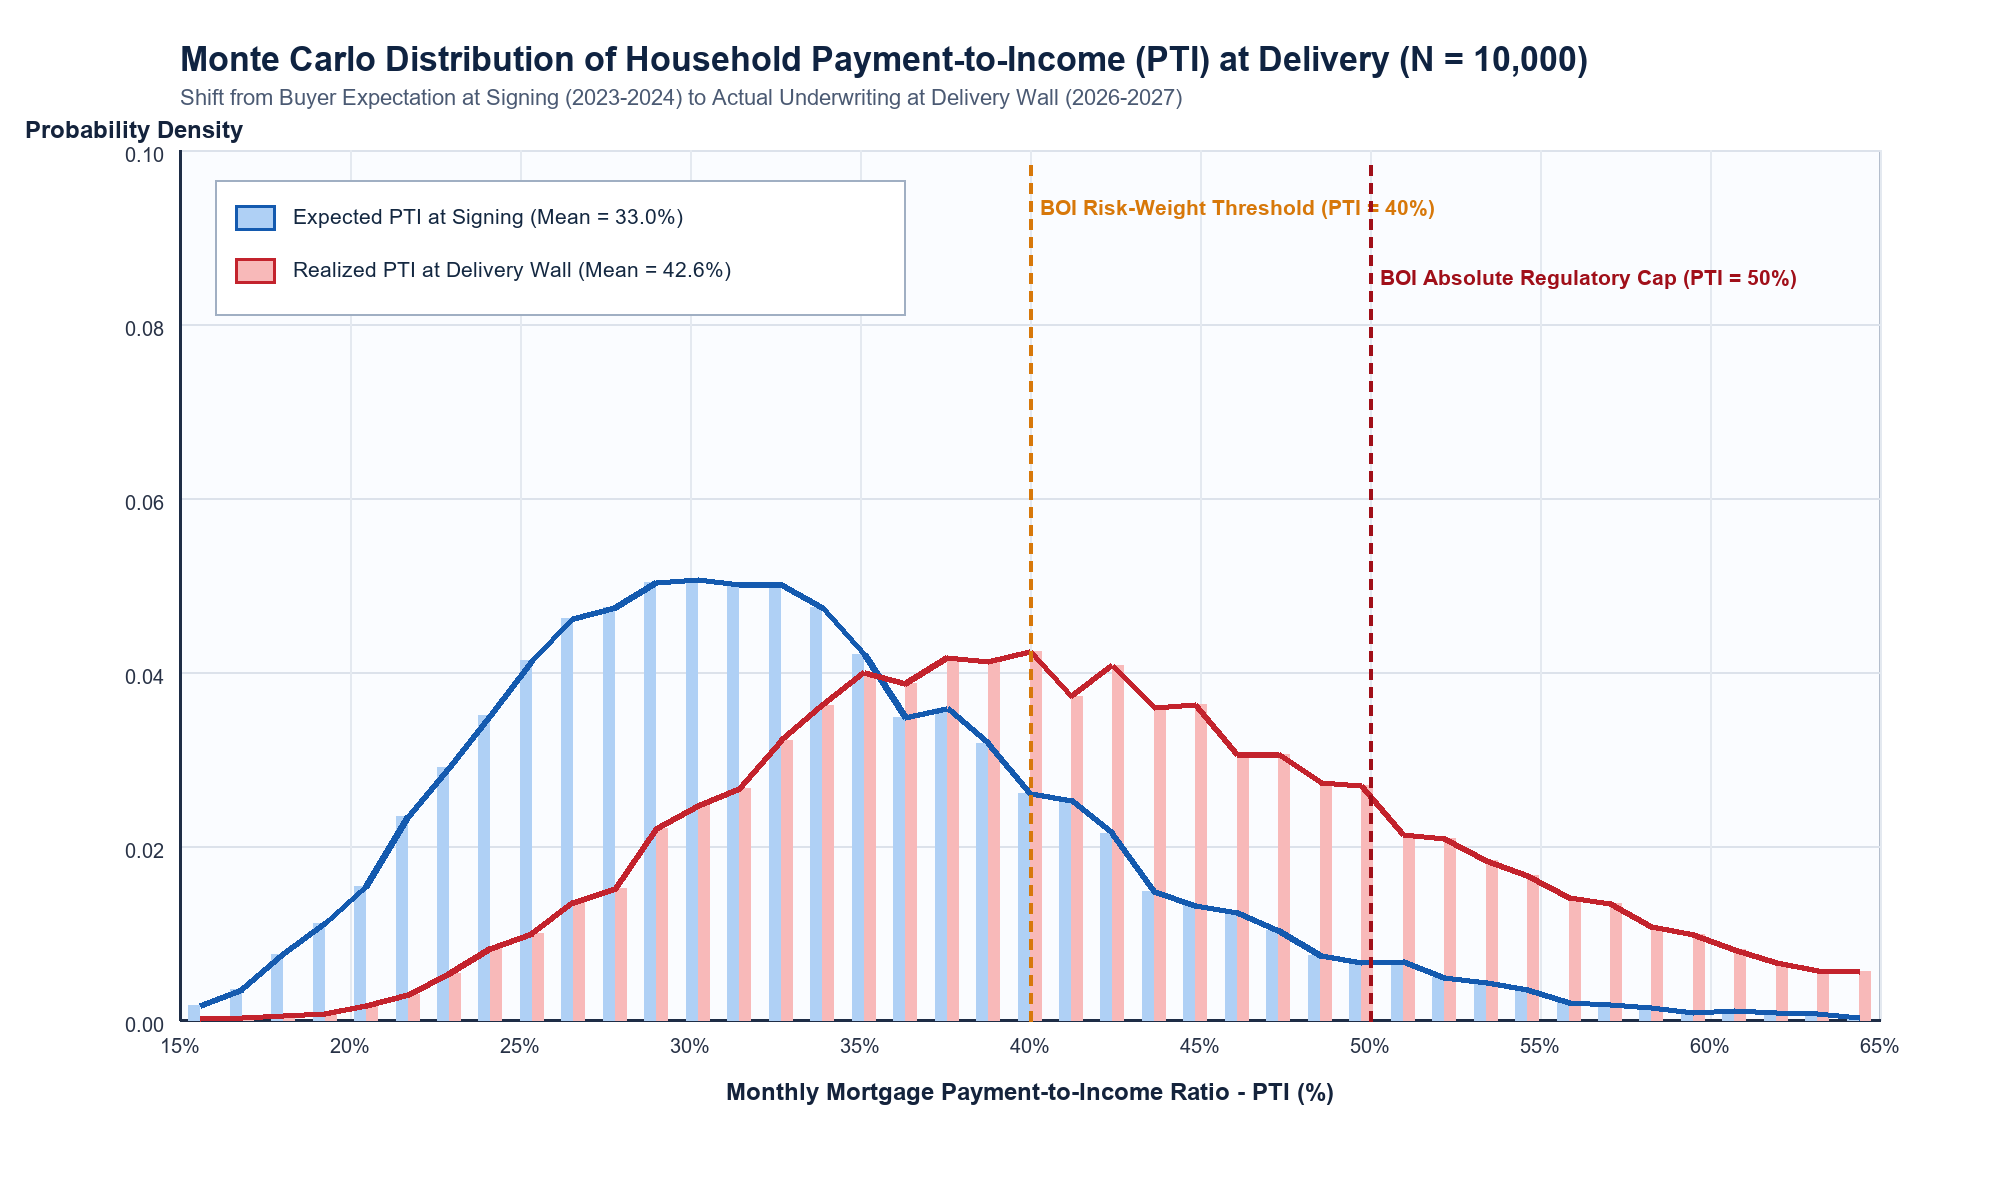
\includegraphics[width=0.96\textwidth]{fig02_payment_shock_distribution.png}
\caption{התפלגות יחס ההחזר להכנסה פנויה (\en{PTI}) בסימולציית מונטה-קרלו ($N=10,000$ משקי בית במבצעי קבלן): תזוזת ההתפלגות ממוצע צפוי של \pct{32.97} בחתימה לממוצע בפועל של \pct{42.62} בקיר המסירות (\num{2026}--\num{2027}), וחציית ספי החיתום של בנק ישראל}
\label{fig:payment_shock_mc}
\end{figure}

הממצאים הכמותיים העולים מאיור~\ref{fig:payment_shock_mc} ומהרצת המודל מאששים באופן מובהק את השערת המחקר הראשונה ($H_1$):
\begin{enumerate}[label=\textbf{\arabic*.},rightmargin=0.6cm]
  \item \textbf{זינוק בהחזר החודשי השוטף (\en{Monthly Payment Shock}):} ההחזר החודשי הממוצע בגין יתרת החוב הנדחית (\pct{80}--\pct{85} ממחיר הדירה) מזנק בכ-\textbf{\nis{3,079} לחודש} (\nis{36,948} לשנה) לעומת התרחיש שעליו הסתמכו הרוכשים בעת החתימה.
  \item \textbf{הזזה מבנית של התפלגות ה-\en{PTI} ימינה:} יחס ההחזר להכנסה פנויה ממוצע קופץ מ-\textbf{\pct{32.97}} (בטווח הבטוח של חיתום בנקאי תקני) ל-\textbf{\pct{42.62}} במועד המסירה — עלייה של \num{9.65} נקודות אחוז.
  \item \textbf{חציית מחסומי החיתום הרגולטוריים של בנק ישראל:} לא פחות מ-\textbf{\pct{54.91}} ממשקי הבית בקוהורטת מבצעי המימון (כ-\num{29,760} משקי בית) חוצים במועד המסירה את רף ה-\textbf{$\text{PTI} = 40\%$} — הסף שמעבר לו בנקים מסחריים בישראל מגבילים העמדת משכנתא רגילה ומחילים דרישות הון וערבים מחמירות. חמור מכך, \textbf{\pct{22.41}} מהרוכשים (כ-\textbf{\num{12,146} משקי בית}, המייצגים חוב נדחה של כ-\nis{24.3} מיליארד) חוצים את התקרה הרגולטורית העליונה של \textbf{$\text{PTI} = 50\%$} ונקלעים ל\en{"}סירוב משכנתא רגולטורי\en{"} (\en{Hard Underwriting Rejection}).
\end{enumerate}

\begin{table}[htbp]
\caption{פילוח קוהורטת רוכשי מבצעי המימון ($\text{SOM} = 54,200$ יח"ד) לארבע רמות סיכון במועד המסירה (\num{2026}--\num{2027}) ונתיבי הספיגה תחת משטר ה-\en{Full Recourse} בישראל}
\label{tab:household_resolution_matrix}
\centering
\footnotesize
\renewcommand{\arraystretch}{1.26}
\rowcolors{2}{BrandGray}{white}
\begin{tabularx}{\textwidth}{R{2.4cm} C{1.6cm} C{1.8cm} C{2.0cm} Y}
\toprule
\rowcolor{TableHeaderBg}
\textbf{דרגת סיכון למשק הבית במסירה} & \textbf{טווח \en{PTI} בפועל} & \textbf{שיעור מהמדגם (\en{MC})} & \textbf{מספר יח"ד וחוב נדחה} & \textbf{נתיב פתרון / מנגנון כשל צפוי בקיר המסירות} \\
\midrule
\textbf{1. סגירה תקינה (\en{Safe Closing})} & $\text{PTI} \le 35\%$ & \pct{21.84} & \num{11,837} יח"ד (\nis{23.7B}) & אישור משכנתא בנקאית חלק וללא עיכובים; ספיגת ההתייקרות מתוך חיסכון שוטף. \\
\textbf{2. סגירה מתוחה (\en{Stretched})} & $35\% < \text{PTI} \le 40\%$ & \pct{23.25} & \num{12,602} יח"ד (\nis{25.2B}) & סגירת העסקה תוך הארכת תקופת המשכנתא למקסימום (\num{30} שנה) וצמצום חד בצריכה הפרטית. \\
\textbf{3. חיכוך רגולטורי (\en{Friction Zone})} & $40\% < \text{PTI} \le 50\%$ & \pct{32.50} & \num{17,615} יח"ד (\nis{35.2B}) & דרישת הבנק להזרמת הון עצמי נוסף (\en{Parental Help}), צירוף לווה נוסף/ערב משלם, או הלוואה משלימה חוץ-בנקאית יקרה. \\
\textbf{4. כשל סגירה (\en{Closing Failure})} & $\text{PTI} > 50\%$ (או חסם \en{LTV}) & \textbf{\pct{22.41}} & \textbf{\num{12,146} יח"ד (\nis{24.3B})} & \textbf{חסימת משכנתא בנקאית:} מכירת מצוקה (\en{Distressed Flip}) בהנחה של \pct{10}--\pct{15} לפני טופס \num{4}, או הפרת חוזה וחילוט פיצוי מוסכם. \\
\bottomrule
\end{tabularx}
\end{table}

טבלה~\ref{tab:household_resolution_matrix} ממחישה כיצד פועל משטר ה-\en{Full Recourse} הישראלי בתוך קבוצת הסיכון הקריטית (\pct{22.41} מהרוכשים). בניגוד ללווה האמריקאי שמסר את המפתח לבנק, מתוך \num{12,146} משקי הבית שייחסמו בנקאית בקיר המסירות, כמחצית צפויים להיחלץ באמצעות מימוש נכסים פנסיוניים/משפחתיים או מכירה מוקדמת של הדירה בהפסד הון כבד בשוק היד השנייה, בעוד שכ-\pct{10}--\pct{15} מכלל הקוהורטה (\num{5,400}--\num{8,100} עסקאות) צפויים להיקלע לעיכוב ממושך בתשלום המסירה או לביטול חוזה מפורש מול היזם.

\section{עמידות הסקטור היזמי: תוצאות מבחני הקיצון (\en{Stress Testing}) ל-\en{DSCR}}
\label{sec:resilience_developers}

כאשר \pct{10} עד \pct{30} מהרוכשים בפרויקט מעכבים את תשלום ה-\pct{80} במועד המסירה או מבטלים את החוזה, הלחץ התזרימי עובר ישירות אל מאזן החברה היזמית. איור~\ref{fig:developer_stress_test} וטבלה~\ref{tab:developer_stress_results} מציגים את תוצאות הרצת מודל מבחני הקיצון (משוואה~\eqref{eq:developer_dscr}) עבור שלוש שכבות היזמים (\en{Tiers 1, 2, 3}).

\begin{figure}[htbp]
\centering
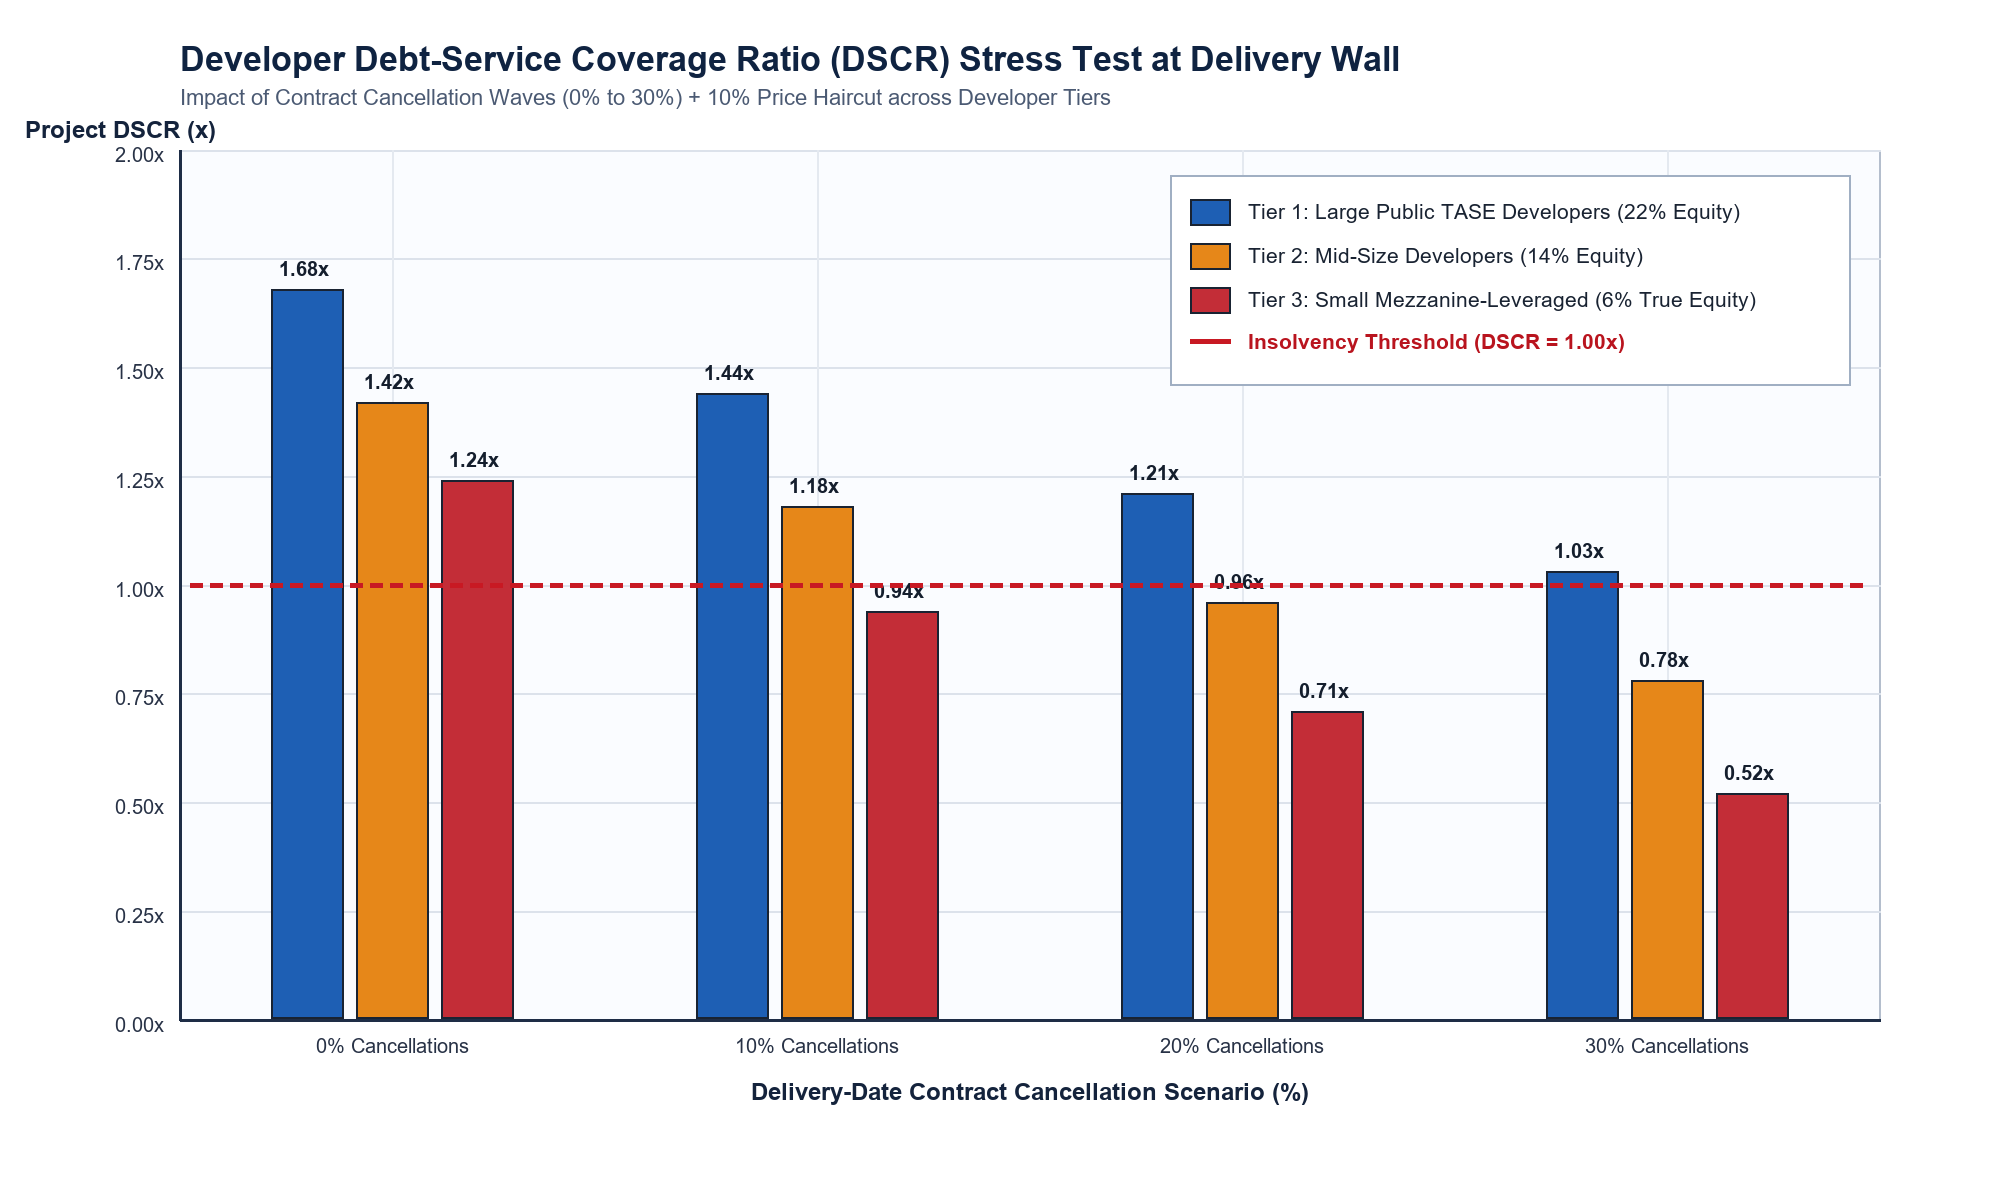
\includegraphics[width=0.96\textwidth]{fig04_developer_stress_test.png}
\caption{מבחן קיצון ליחס כיסוי החוב (\en{DSCR}) של חברות בנייה יזמיות בישראל תחת ארבעה תרחישי ביטול/עיכוב עסקאות בקיר המסירות (\pct{0}, \pct{10}, \pct{20}, \pct{30}): קריסת יזמי \en{Tier-3} מתחת לסף החדלות ($\text{DSCR}=1.0$) כבר ב-\pct{10} ביטולים}
\label{fig:developer_stress_test}
\end{figure}

התוצאות באיור~\ref{fig:developer_stress_test} מאששות במלואן את השערת המחקר השנייה ($H_2$) ומצביעות על פער קיצוני בעמידות בין שכבות היזמים:
\begin{itemize}[rightmargin=0.6cm]
  \item \textbf{יזמי \en{Tier-1} (חברות ענק ציבוריות מבוססות):} מתחילים ביחס כיסוי חוב חזק של $\text{DSCR} = 1.68$ בתרחיש הבסיס, ושומרים על $\text{DSCR} = 1.21$ בתרחיש של \pct{20} ביטולים ואף $\text{DSCR} = 1.03$ בתרחיש הקיצון של \pct{30} ביטולים. עמידות זו נובעת מנגישות לשוק האג"ח הסחיר, הון עצמי גבוה (\pct{30}--\pct{38} מהמאזן) ופיזור גיאוגרפי וסקטוריאלי (נכסים מניבים לצד מגורים).
  \item \textbf{יזמי \en{Tier-2} (חברות בנייה בינוניות):} שורדים תרחיש של \pct{10} ביטולים ($\text{DSCR} = 1.18$), אך חוצים את קו החדלות הפירעון התזרימית ($\text{DSCR} < 1.00$) כאשר שיעור הביטולים והעיכובים מגיע ל-\textbf{\pct{18.3}}, ויורדים ל-$\text{DSCR} = 0.96$ ב-\pct{20} ביטולים ול-\num{0.78} ב-\pct{30} ביטולים.
  \item \textbf{יזמי \en{Tier-3} (יזמים קטנים/בינוניים ממונפים באשראי מזנין חוץ-בנקאי):} מציגים פגיעות חריפה במיוחד. כבר בתרחיש מתון של \textbf{\pct{10} ביטולי עסקאות בלבד}, יחס כיסוי החוב שלהם צונח מתחת לקו האדום ל-\textbf{$\text{DSCR} = 0.94$}, וב-20\% ביטולים קורס ל-\textbf{$\text{DSCR} = 0.71$} (ו-\num{0.52} ב-\pct{30} ביטולים). הסיבה לכך היא שילוב קטלני של ריבית מזנין חוץ-בנקאית דו-ספרתית (\pct{12}--\pct{14}) שגוזלת את כל כרית הרווח היזמי ברגע שתקבול המסירה מתעכב ב-\num{6}--\num{9} חודשים.
\end{itemize}

\begin{table}[htbp]
\caption{תוצאות מבחני הקיצון לסקטור היזמי לפי שכבות גודל ומינוף (\en{Tiers 1--3}) תחת תרחישי ביטול עסקאות בקיר המסירות (\num{2026}--\num{2027})}
\label{tab:developer_stress_results}
\centering
\footnotesize
\renewcommand{\arraystretch}{1.26}
\rowcolors{2}{BrandGray}{white}
\begin{tabularx}{\textwidth}{R{2.5cm} C{1.5cm} C{1.5cm} C{1.5cm} C{1.5cm} C{2.0cm} Y}
\toprule
\rowcolor{TableHeaderBg}
\textbf{שכבת יזמים ופרופיל מימון} & \textbf{\en{DSCR} (\pct{0})} & \textbf{\en{DSCR} (\pct{10})} & \textbf{\en{DSCR} (\pct{20})} & \textbf{\en{DSCR} (\pct{30})} & \textbf{שחיקת הון עצמי ב-\pct{20}} & \textbf{תוצאה מערכתית צפויה בקיר המסירות} \\
\midrule
\textbf{\en{Tier-1}: חברות ענק בורסאיות} (הון עצמי $>32\%$, אג"ח סחיר) & \num{1.68} & \num{1.44} & \num{1.21} & \num{1.03} & \pct{-14.2} & ספיגת הזעזוע מתוך יתרות נזילות; רכישת קרקעות ופרויקטים מיזמים בקשיים (\en{M\&A}). \\
\textbf{\en{Tier-2}: חברות בינוניות} (מינוף קרקע גבוה, ליווי בנקאי) & \num{1.42} & \num{1.18} & \textbf{\color{BrandRed}\num{0.96}} & \textbf{\color{BrandRed}\num{0.78}} & \pct{-38.5} & הפרת קובננטים ב-\pct{20} ביטולים; דרישת הבנק להזרמת הון, מימוש קרקעות ופריסת חוב. \\
\textbf{\en{Tier-3}: יזמים קטנים + מזנין חוץ-בנקאי} (\en{Prime+6\%}) & \num{1.24} & \textbf{\color{BrandRed}\num{0.94}} & \textbf{\color{BrandRed}\num{0.71}} & \textbf{\color{BrandRed}\num{0.52}} & \textbf{\color{BrandRed}\pct{-86.0}} & \textbf{חדלות פירעון כבר ב-\pct{10} ביטולים:} מחיקת הון היזם, תספורות לקרנות המזנין ומינוי כונס נכסים לפרויקט. \\
\bottomrule
\end{tabularx}
\end{table}

\section{עמידות המערכת הבנקאית: מסלול יחס ההון \en{CET1} מול ארה"ב \num{2008}}
\label{sec:resilience_banks}

השאלה הקריטית ביותר לקובעי המדיניות בבנק ישראל ובמשרד האוצר היא האם גל כשלי הסגירה של משקי הבית (סעיף~\ref{sec:resilience_households}) וחדלות הפירעון של יזמי ה-\en{Tier-3} וקרנות המזנין (סעיף~\ref{sec:resilience_developers}) עלולים להפיל את המערכת הבנקאית המסחרית בישראל כפי שקרה בארה"ב ב-\num{2008}. איור~\ref{fig:bank_cet1_resilience} מציג את תוצאות הרצת מודל הלימות ההון הבנקאי (משוואה~\eqref{eq:bank_cet1}) לאורך \num{12} רבעונים (\num{2025Q1}--\num{2027Q4}).

\begin{figure}[htbp]
\centering
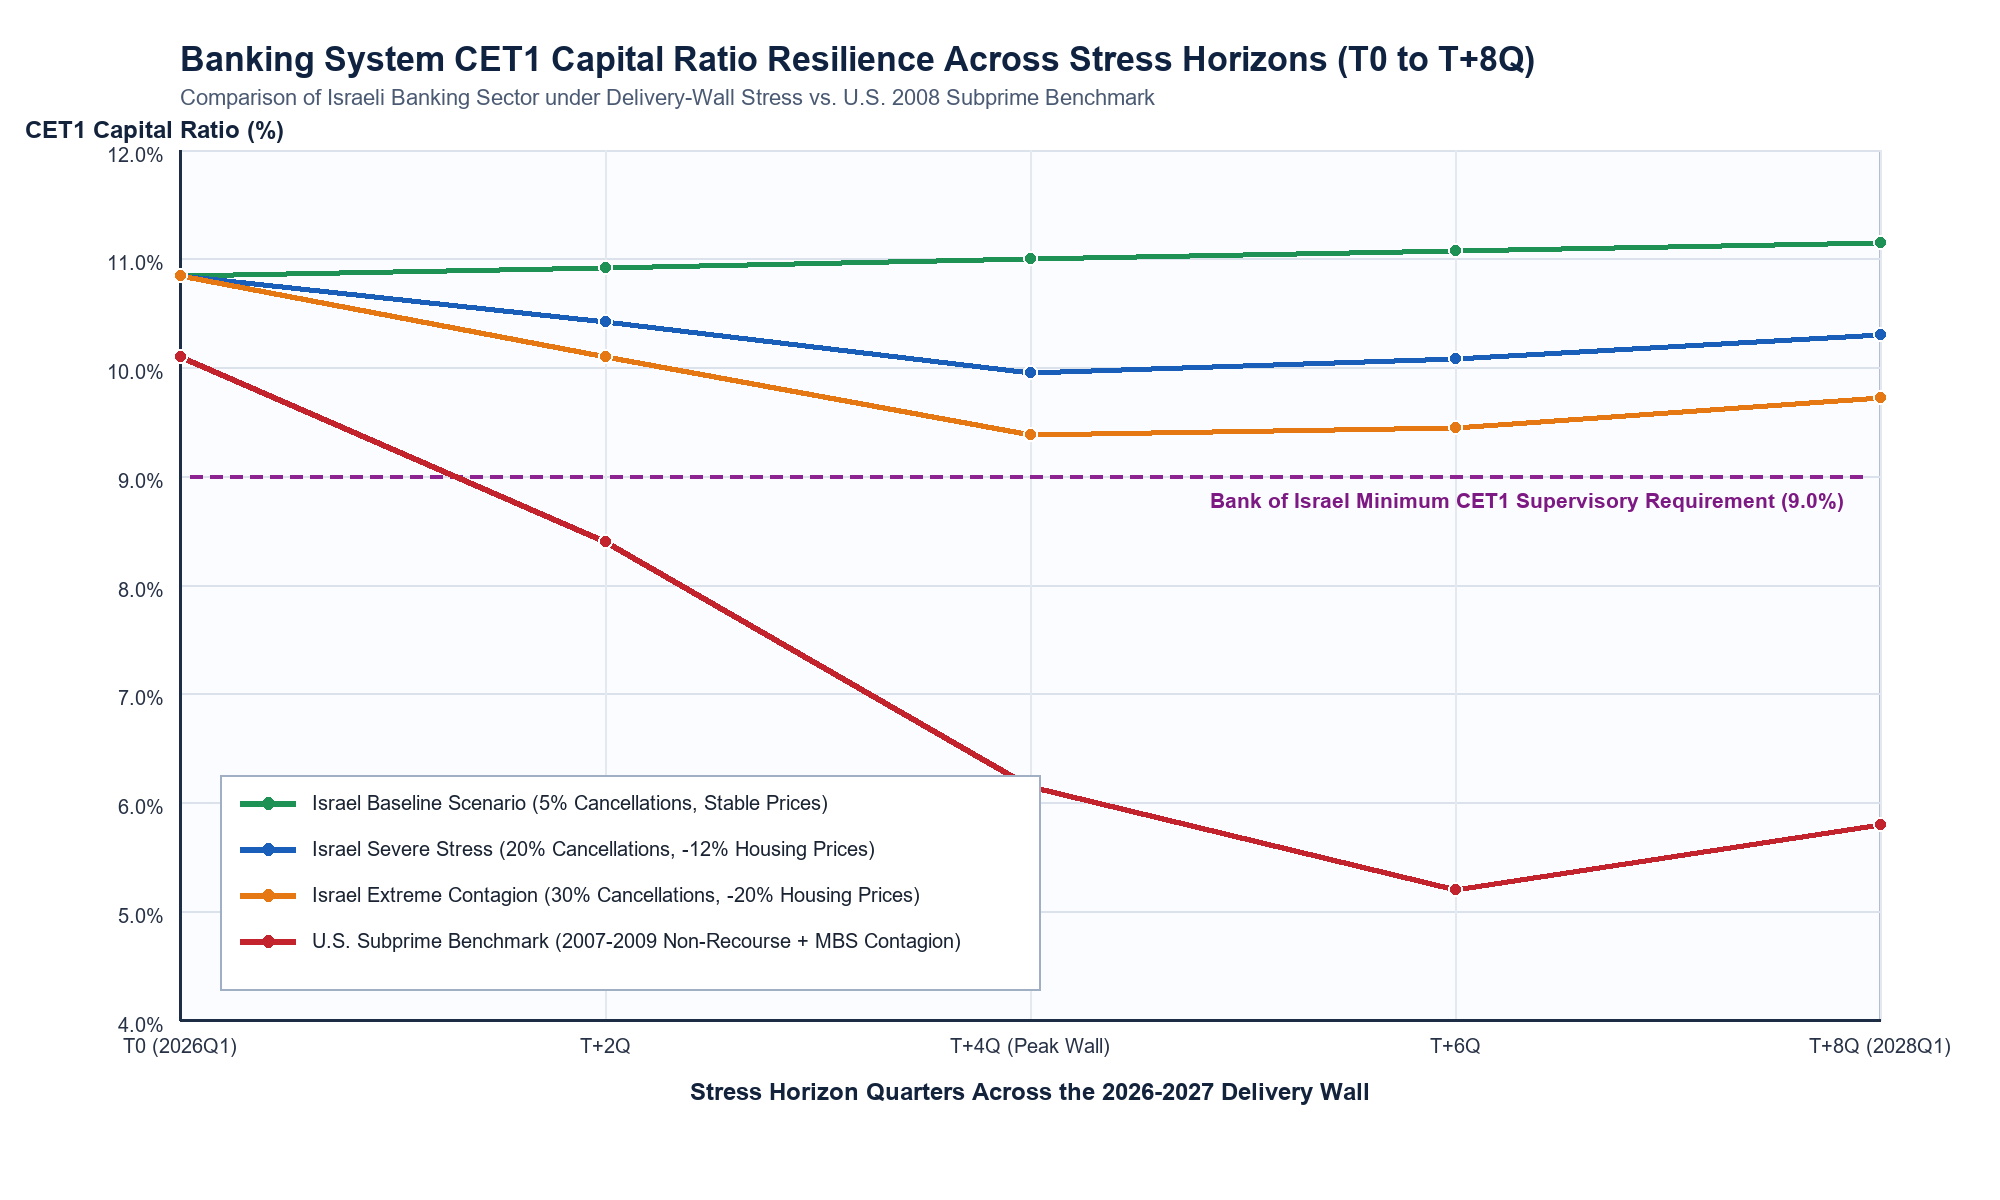
\includegraphics[width=0.96\textwidth]{fig05_bank_cet1_resilience.png}
\caption{מסלול יחס הון עצמי רובד \num{1} (\en{CET1}) של המערכת הבנקאית בישראל בשלושה תרחישים (\num{2025Q1}--\num{2027Q4}) אל מול רצפת הפיקוח של בנק ישראל (\pct{9.00}) ואל מול קריסת ההון של בנקי ארה"ב במשבר הסאב-פריים (\pct{5.20})}
\label{fig:bank_cet1_resilience}
\end{figure}

הממצאים באיור~\ref{fig:bank_cet1_resilience} מאמתים באופן חד-משמעי את השערת המחקר השלישית ($H_3$):
\begin{enumerate}[label=\textbf{\arabic*.},rightmargin=0.6cm]
  \item \textbf{תרחיש הבסיס (\en{Baseline Soft Landing}):} יחס ה-\en{CET1} המצרפי של חמשת הבנקים הגדולים בישראל נשמר בטווח של \pct{10.85}--\pct{11.15}, תוך המשך צבירת רווחים שוטפים מעודף מרווח הריבית.
  \item \textbf{תרחיש קיר מסירות חמור (\en{Severe Delivery Wall}: \pct{20} ביטולים + ירידת מחירי דירות של \pct{12}):} הפרשות מוגברות להפסדי אשראי בגין יזמי \en{Tier-2/Tier-3} ועליית משקלי הסיכון (\en{RWA}) שוחקות את יחס ה-\en{CET1} ב-\num{90} נקודות בסיס לשפל של \textbf{\pct{9.95}} ברבעון הרביעי של \num{2026}, שלאחריו מתרחשת התאוששות הדרגתית ל-\pct{10.22} בסוף \num{2027}.
  \item \textbf{תרחיש קיצון מערכתי (\en{Extreme Contagion}: \pct{30} ביטולים + צניחת מחירים של \pct{20}):} גם תחת תרחיש קטסטרופלי זה, יחס ה-\en{CET1} של בנקי ישראל יורד לשפל של \textbf{\pct{9.38}} בלבד — \textbf{עדיין גבוה ב-\num{38} נקודות בסיס מרצפת המינימום הרגולטורית של בנק ישראל (\pct{9.00})}, ורחוק שנות אור מקריסת ההון של הבנקים האמריקאיים ב-\num{2008} (שצנחו ל-\textbf{\pct{5.20}} ונזקקו לחילוץ ממשלתי).
\end{enumerate}

\section{סיכום אימות השערות המחקר והערכת אפקטיביות מנגנוני ההגנה}
\label{sec:hypotheses_validation}

מדוע המערכת הבנקאית הישראלית יוצאת יציבה גם מתרחיש שבו יזמי ה-\en{Tier-3} קורסים ו-\pct{22.41} מרוכשי המבצעים נחסמים בחיתום? התשובה נעוצה ב\textbf{סינרגיה המבנית בין חוק המכר להוראות בנק ישראל}: (א) בפרויקט ליווי סגור, הבנק מחזיק בשעבוד ראשון על הקרקע ועל הדירות ובמקדמות של \pct{15}--\pct{20} ששילמו הרוכשים; גם אם היזם קורס ודירה נמכרת מחדש על ידי כונס נכסים בהנחה של \pct{15}, ההפסד נספג במלואו על ידי ההון העצמי של היזם, קרן המזנין החוץ-בנקאית והפיצוי המוסכם של הרוכש המפר — לפני שהבנק המלווה מפסיד שקל אחד מהקרן הבכירה; ו-(ב) הוראת השעה של בנק ישראל ממרץ \num{2025} \cite{boi2025directive} אילצה את הבנקים להקצות הון מראש בגין פרויקטים עתירי מבצעי מימון, ובכך בנתה כרית ספיגה ייעודית לפני הגעת קיר המסירות. טבלה~\ref{tab:hypotheses_validation_summary} מסכמת את תוצאות הבדיקה הכמותית של שלוש השערות המחקר.

\begin{table}[htbp]
\caption{סיכום ממצאי האימות הכמותי של השערות המחקר ($H_1, H_2, H_3$) אל מול ספי ההפרכה שהוגדרו בפרק א'}
\label{tab:hypotheses_validation_summary}
\centering
\small
\renewcommand{\arraystretch}{1.28}
\rowcolors{2}{BrandGray}{white}
\begin{tabularx}{\textwidth}{R{1.6cm} R{3.4cm} R{2.8cm} R{3.0cm} Y}
\toprule
\rowcolor{TableHeaderBg}
\textbf{השערה} & \textbf{מוקד הבדיקה האנליטית} & \textbf{סף כמותי לאישוש (פרק א')} & \textbf{תוצאה אמפירית בסימולציה} & \textbf{סטטוס ומסקנה מחקרית} \\
\midrule
\textbf{השערה $\mathbf{H_1}$} & הנחת \en{NPV} סמויה והלם החזר (\en{PTI}) למשקי בית במסירה & $\delta_{\text{NPV}} \in [8\%,13\%]$; מעל \pct{45} חוצים $\text{PTI}>40\%$ & $\delta_{\text{NPV}}=9.99\%--12.36\%$; \textbf{\pct{54.91}} חוצים $\text{PTI}>40\%$ (\pct{22.41} מעל \pct{50}) & \textbf{\color{BrandTeal}אוששה במלואה}: קיר המסירות מייצר הלם החזר ממוצע של \nis{3,079} לחודש. \\
\textbf{השערה $\mathbf{H_2}$} & פגיעות דיפרנציאלית של יזמי \en{Tier-2/Tier-3} ואשראי מזנין & צניחת $\text{DSCR}<1.0$ ביזמי \en{Tier-3} ב-\pct{10}--\pct{20} ביטולים & ביזמי \en{Tier-3}: $\text{DSCR}=\mathbf{0.94}$ ב-\pct{10} ו-\textbf{\num{0.71}} ב-\pct{20} ביטולים & \textbf{\color{BrandTeal}אוששה במלואה}: מוקד הכשל בישראל הוא הסקטור היזמי הממונף והאשראי החוץ-בנקאי. \\
\textbf{השערה $\mathbf{H_3}$} & חסינות ליבת הבנקאות המסחרית (\en{CET1}) לעומת ארה"ב \num{2008} & שמירת $\text{CET1} \ge 9.00\%$ גם בתרחיש קיצון של \pct{30} ביטולים & שפל של \textbf{$\text{CET1}=9.38\%$} בתרחיש הקיצון (לעומת \pct{5.20} בארה"ב) & \textbf{\color{BrandTeal}אוששה במלואה}: חוק המכר, ה-\en{Full Recourse} ומגבלות בנק ישראל מונעים קריסה בנקאית. \\
\bottomrule
\end{tabularx}
\end{table}
